\subsection{Logiciel utilisé}
\subsubsection{Snap!}
\url{http://snap.berkeley.edu/SnapManual.pdf}
Cet partie va donner un aperçu de l'application réutilisée dans ce travail, à savoir Snap!. Comme dit précédemment, cette application est réalisée en JavaScript. La présentation de Snap! va se diviser en plusieurs partie. La première expliquera les différents types de blocs et comment ils sont implémentés. L'exécution d'un programme est l'étape suivante. Enfin, il sera présenté comment l'application affiche les différents éléments la constituant.

\paragraph{Blocs}
Il existe plusieurs type de blocs qui constitue un programme Snap!. Sur l'exemple de programme \ref{fig:software_used_script}, les différents type blocs disponible sont présenté.
\begin{figure}
  \begin{center}
    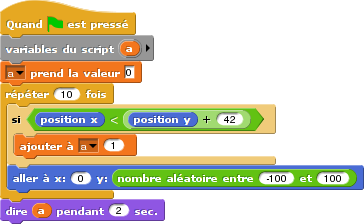
\includegraphics[width=0.5\textwidth]{content/4-theory/2-related_work/images/script}
    \caption{Exemple de programme Snap!}
    \label{fig:software_used_script}
  \end{center}
\end{figure}

\subparagraph{Commande}
Le principal type de bloc est la commande. Ces blocs peuvent être compris comme étant des procédures. En effet, les blocs exécutes une ou plusieurs opérations sur le système en fonction des paramètres passé. Ces différents blocs doivent se baser soit sur une implémentation JavaScript pour les commandes élémentaires, soit être une composition de commandes pour fournir une commande plus complète et/ou abstraite.

Dans l'exemple \ref{fig:software_used_script}, ce sont tout les blocs qui on la forme d'une pièce de puzzle. On peut voir que l'on a une succession de commandes qui crée un script. Les commandes ont plusieurs couleurs suivant la catégorie à laquel elles appartiennent : mouvement, apparence, contrôles, variable\ldots

\subparagraph{Reporter}
Les reporters sont des fonctions. En effet, il retourne une valeur. Ils sont toujours utilisé en temps que parametres d'un autre bloc. La plupart des reporter sont des accesseurs à des variables ou à des états du système (position souris, heure \ldots). 

Les reporters sont les blocs de forme arrondie. L'exemple \ref{fig:software_used_script} montre différente utilisation de reporters : somme, valeur aléatoire, position \ldots Tout comme pour les commandes, les reporters peuvent être de différente couleur suivant leur catégorie.

\subparagraph{Prédicat}
Les prédicats sont des reporters qui retourne une valeur booléenne. Ils sont donc utilisé en conjonction avec des commandes demandant une condition.

Les prédicats sont les blocs de forme hexagonale.

\subparagraph{Chapeau}
Les chapeaux sont des commandes spéciales car ils sont le point d'entrée obligatoire d'un script. Ils permettent de démarrer l'exécution d'un script quand un événement se produit.

L'événement qui lancera le script \ref{fig:software_used_script} est donc le démarrage du programme. Celui-ci est symbolisé par un bouton avec drapeau vert.

\paragraph{Programme}
Snap! est plus qu'une interface graphique permettant de construire un programme. L'analyse du fonctionnement interne est l'object de cette section.

Un programme est constitué de plusieurs processus. Chaque processus sera exécuté en parallèle grace à un ordonanceur.

% /*
%     A Process is what brings a stack of blocks to life. The process
%     keeps track of which block to run next, evaluates block arguments,
%     handles control structures, and so forth.
% 
%     The ThreadManager is the (passive) scheduler, telling each process
%     when to run by calling its runStep() method. The runStep() method
%     will execute some number of blocks, then voluntarily yield control
%     so that the ThreadManager can run another process.
% 
%     The Scratch etiquette is that a process should yield control at the
%     end of every loop iteration, and while it is running a timed command
%     (e.g. "wait 5 secs") or a synchronous command (e.g. "broadcast xxx
%     and wait"). Since Snap also has lambda and custom blocks Snap adds
%     yields at the beginning of each non-atomic custom command block
%     execution, and - to let users escape infinite loops and recursion -
%     whenever the process runs into a timeout.
% 
%     a Process runs for a receiver, i.e. a sprite or the stage or any
%     blocks-scriptable object that we'll introduce.
% 
%     structure:
% 
%     topBlock            the stack's first block, of which all others
%                         are children
%     receiver            object (sprite) to which the process applies,
%                         cached from the top block
%     context                the Context describing the current state
%                         of this process
%     homeContext            stores information relevant to the whole process,
%                         i.e. its receiver, result etc.
%     isPaused            boolean indicating whether to pause
%     readyToYield        boolean indicating whether to yield control to
%                         another process
%     readyToTerminate    boolean indicating whether the stop method has
%                         been called
%     isDead              boolean indicating a terminated clone process
%     timeout                msecs after which to force yield
%     lastYield            msecs when the process last yielded
%     errorFlag            boolean indicating whether an error was encountered
%     prompter            active instance of StagePrompterMorph
%     httpRequest         active instance of an HttpRequest or null
%     pauseOffset         msecs between the start of an interpolated operation
%                         and when the process was paused
% */

Un processus \texttt{Process} représente l'exécution d'un script, une pile de blocs. Il assure le suivit de l'exécution du script : prochain bloc à s'executer, object sur lequel il s'applique (lutin, stage), contexte décrivant l'état courant \ldots

L'ordonanceur \texttt{ThreadManager} appelle sucessivement la fonction \texttt{runStep()} (\ref{lst-runstep}) sur chaque processus. Cette fonction exécute un certain nombre de blocs via \texttt{this.evaluateContext()} de manière atomique. Elle rend la main volontairement à l'ordonanceur quand elle a terminé. Comme il est possible d'écrire soi-même des blocs, \texttt{runStep()} rend aussi la main si trop de temps s'est écoulé depuis le début de l'exécution de cette étape. La convention est que les processus rendent la main à la fin de chaque itération de boucle ou quand une opération relative au temps (attendre xxx secondes) ou synchrone (envoyer à tous xxx et attendre la réponse) est exécutée.

\begin{lstlisting}[caption={Fonction \texttt{runStep()} de \texttt{Process}},label=lst-runstep,language=JavaScript]
Process.prototype.runStep = function () {
/*
    a step is an an uninterruptable 'atom', it can consist
    of several contexts, even of several blocks
*/
    // allow pausing in between atomic steps:
    if (this.isPaused) {
        return this.pauseStep();
    }
    this.readyToYield = false;
    while (!this.readyToYield
            && this.context
            && (this.isAtomic ? (Date.now() - this.lastYield < this.timeout) : true) ) {
        // also allow pausing inside atomic steps - for PAUSE block primitive:
        if (this.isPaused) {
            return this.pauseStep();
        }
        this.evaluateContext();
    }
    this.lastYield = Date.now();

    // make sure to redraw atomic things
    if (this.isAtomic &&
            this.homeContext.receiver &&
            this.homeContext.receiver.endWarp) {
        this.homeContext.receiver.endWarp();
        this.homeContext.receiver.startWarp();
    }

    if (this.readyToTerminate) {
        while (this.context) {
            this.popContext();
        }
        // pen optimization
        if (this.homeContext.receiver &&
                this.homeContext.receiver.endWarp) {
            this.homeContext.receiver.endWarp();
        }
    }
};
\end{lstlisting}



% /*
%     A Context describes the state of a Process.
% 
%     Each Process has a pointer to a Context containing its
%     state. Whenever the Process yields control, its Context
%     tells it exactly where it left off.
% 
%     structure:
% 
%     parentContext    the Context to return to when this one has
%                     been evaluated.
%     outerContext    the Context holding my lexical scope
%     expression        SyntaxElementMorph, an array of blocks to evaluate,
%                     null or a String denoting a selector, e.g. 'doYield'
%     receiver        the object to which the expression applies, if any
%     variables        the current VariableFrame, if any
%     upvars          the current UpvarReference, if any (default: null)
%     inputs            an array of input values computed so far
%                     (if expression is a    BlockMorph)
%     pc                the index of the next block to evaluate
%                     (if expression is an array)
%     startTime        time when the context was first evaluated
%     startValue        initial value for interpolated operations
%     activeAudio     audio buffer for interpolated operations, don't persist
%     activeNote      audio oscillator for interpolated ops, don't persist
%     isLambda        marker for return ops
%     isImplicitLambda    marker for return ops
%     isCustomBlock   marker for return ops
%     emptySlots        caches the number of empty slots for reification
% */

\paragraph{GUI}
Un autre élément interessant à analyser chez Snap! est sa facon d'afficher quelque chose dans la balise html \texttt{canvas}. Toutes les fonctionnalités de base nécessaire à afficher tout éléments graphiques (text rendering, blinking cursors, entry fields, menus, buttons, sliders, windows and dialog boxes \ldots) de Snap! découle de l'implémentation que l'on retrouve dans \texttt{morphic.js}.

\texttt{morphic.js} fournit les abstractions nécessairent à redessiner des parties de l'interface et pour interagir avec l'utilisateur. Le canvas utilisé possède un \texttt{world}. Ce \texttt{world} est la racine de l'arbre composé de \texttt{morph} et leur sous-\texttt{morph}. Chaque \texttt{morph} peut être déplacé, redimentionné via le code ou les manipulations de l'utilisateurs.

L'idée principale de \texttt{morphic.js} est de continuellement parcourir tout les éléments du \texttt{world} pour redessiner ceux qui ont été modifié. Le \texttt{world} permet à l'ordonnanceur d'exécuter une étape entre chaque itération. L'exemple \ref{lst-doonecycle} que le monde est rafraichit toutes les 50ms.

\begin{lstlisting}[caption={Exemple d'utilisation de \texttt{morphic.js}},label=lst-doonecycle,language=HTML5,alsolanguage=JavaScript]
<!DOCTYPE html>
<html>
    <head>
        <title>Morphic!</title>
        <script type="text/javascript" src="morphic.js"></script>
        <script type="text/javascript">
            var world;

            window.onload = function () {
                world = new WorldMorph(
                    document.getElementById('world'));
                setInterval(loop, 50);
            };

            function loop() {
                world.doOneCycle();
            }
        </script>
    </head>
    <body>
        <canvas id="world" tabindex="1" width="800" height="600" />
    </body>
</html>
\end{lstlisting}

La fonction \texttt{drawNew()} sert dessiner un \texttt{morph}. L'exemple \ref{lst-drawnew} montre que cette fonction dessine son objet sur une image stockée dans l'objet. Cette image provient d'un canvas virtuel généré grace à l'image du \texttt{morph} parent.

\begin{lstlisting}[caption={Modèle pour la fonction \texttt{drawNew()}},label=lst-drawnew,language=JavaScript]
MyMorph.prototype.drawNew = function() {
    var context;
    this.image = newCanvas(this.extent());
    context = this.image.getContext('2d');
    // use context to paint stuff here
};
\end{lstlisting}

\subsubsection{Rails}
Pour permettre de suivre un étudiant et de faire intéragir le professeur dans le dévelopement, un pe platforme web est nécessaire. Ruby on Rails est le framework choisi pour déveloper l'application web. 

\paragraph{Philosophie}
Rails fait l'assomption qu'il existe une meilleur facon d'aborder la création d'application web. Si le programmeur respect ce "Rails way", il amméliorera sa productivité et écrira moins de code. Par contre si il persiste à utiliser ses anciennes habitudes, il aura beaucoup moins d'amusement à déveloper une application.

Pour atteindre cet objectif, Rails utilise deux principes majeurs :
\begin{description}
  \item[convention plutot que configuration] (CoC) Pour permettre au programmeur d'écrire moins de code, Rails permet de n'écrire que ce qui ne correspond pas aux conventions. Rails utilise la métaprogrammation pour fournir les conventions à tous objets.
  \item[ne vous répétez  pas] (DRY) L'architecture que propose Rails permet de mettre l'information à un endroit unique et bien déterminé. Ceci permet d'avoir un code plus court, plus maintenable, plus extensible et moins bugé.
\end{description}

\paragraph{architecture}
Rails se base sur une architecture Modèle-Vue-Controlleur.
\subparagraph{Modèle} 
Un modèle est typiquement une classe qui représente une table de la base de données. Une classe du modèle fournit aussi toutes les méthode nécessaire à représenter et modifier l'objet dans le domaine d'application.

La correspondance entre un objet Ruby et la base de données est réalisée grâce à Active Record. Ce module de Rails permet de faire des appels sur des objets Ruby alors que dans d'autres framework, il faudrait utiliser des requètes SQL.
  
\subparagraph{Controlleur} 
Le controlleur permet d'accéder à une ressource. Une ressource est un modèle ou toute autre objet plus indirect (enregistrement/login, page d'acceuil\ldots).  

Il détermine quel vue doit s'afficher et avec quel paramètre. Le controlleur a donc la tache de vérifier la sécurité et l'intégrité des données fournies par l'utilisateur. Ensuite, il peut intéroger différents modèles et fournir les réponses à la vue adéquate. 

Rails encourage d'avoir des ressources REST. C'est a dire, d'avoir des ressources avec une représentations unique et des actions identique (create, new, edit, update, destroy, show, index). Les actions disponible sur un controlleur sont déterminées via le fichier de configuration des routes.

\subparagraph{Vue} 
Les vues sont ce que les utilisateurs recoivent et voient. Ce sont typiquement des pages html mais aussi des pdf, objet json, fichier\ldots 

La philosophie de Rails est d'utiliser des gems pour simplifier l'écriture. Pour les vues, nous avons notament:
\begin{description}
  \item[Haml] un langage fournissant une syntaxe raccourcie du html. Il se base sur l'indentation plutot que sur une syntaxe XML. Haml permet donc de respecter le principe DRY et d'amélioré la lisibilité par code plus court et bien indenté.
  \item[JQuery] Cette bibliothèque javascript bien connue permet de ne pas réinventer la roue lorsque l'on veut pouvoir ajouter un peu de dynamisme à nos page web.
  \item[CoffeeScript] Un langage qui se compile en JavaScript. Il permet d'avoir une syntaxe plus claire et plus courte et d'ajouter des sucre syntaxique par raport à JavaScript.
  \item[Bootstrap] un framework CSS qui permet de découpler le fond de la forme de l'affichage d'une page html. Ce framework donne un disign responsive pour tout type d'écran au page qui l'utilise. Il fournit aussi de nombreux composants utiles (boutons, alertes, barre de progression, message d'aide \ldots).
\end{description}

\paragraph{gem}
meme rails est un gem

\begin{description}
  \item[autority / rolify]
  \item[paperclip]
  \item[devise]
\end{description}

\paragraph{test}
\begin{description}
  \item[factory girls]
  \item[cucumber et capybara]
  \item[RSpec]
  \item[Travis]
  \item[Coveralls]
  \item[codeclimate]
  \item[Rails Best Practice] 
\end{description}
